\documentclass[10pt,xcolor={usenames,dvipsnames}]{beamer}

\usetheme[progressbar=frametitle]{metropolis}

\usepackage{booktabs}
\usepackage[scale=2]{ccicons}
\usepackage[geometry]{ifsym}
\usepackage{pgfplots}
\usepackage{multirow}
\usepackage{biblatex}
%\usepgfplotslibrary{dateplot}
%\usepackage[natbib=true,style=authoryear,backend=bibtex,useprefix=true]{biblatex}
%\addbibresource{refepresen.bib}
%\usepackage[backend=biber,style=numeric-comp,sorting=none]{biblatex}

\usepackage{xspace}
\newcommand{\themename}{\textbf{\textsc{metropolis}}\xspace}
\graphicspath{{images/},{figures/}}

 % <--- number references





\title{Análisis estadístico del flujo de 1-gramas entre lenguajes indoeuropeos}
%\subtitle{And all that jazz}
\date{1° julio de 2021}
\author{Josué Ely Molina Becerra}
\institute{Universidad Nacional Autónoma de México
\\ \textbf{Asesor de tesis: Dr. Carlos Francisco Pineda Zorrilla}}
\titlegraphic{\hfill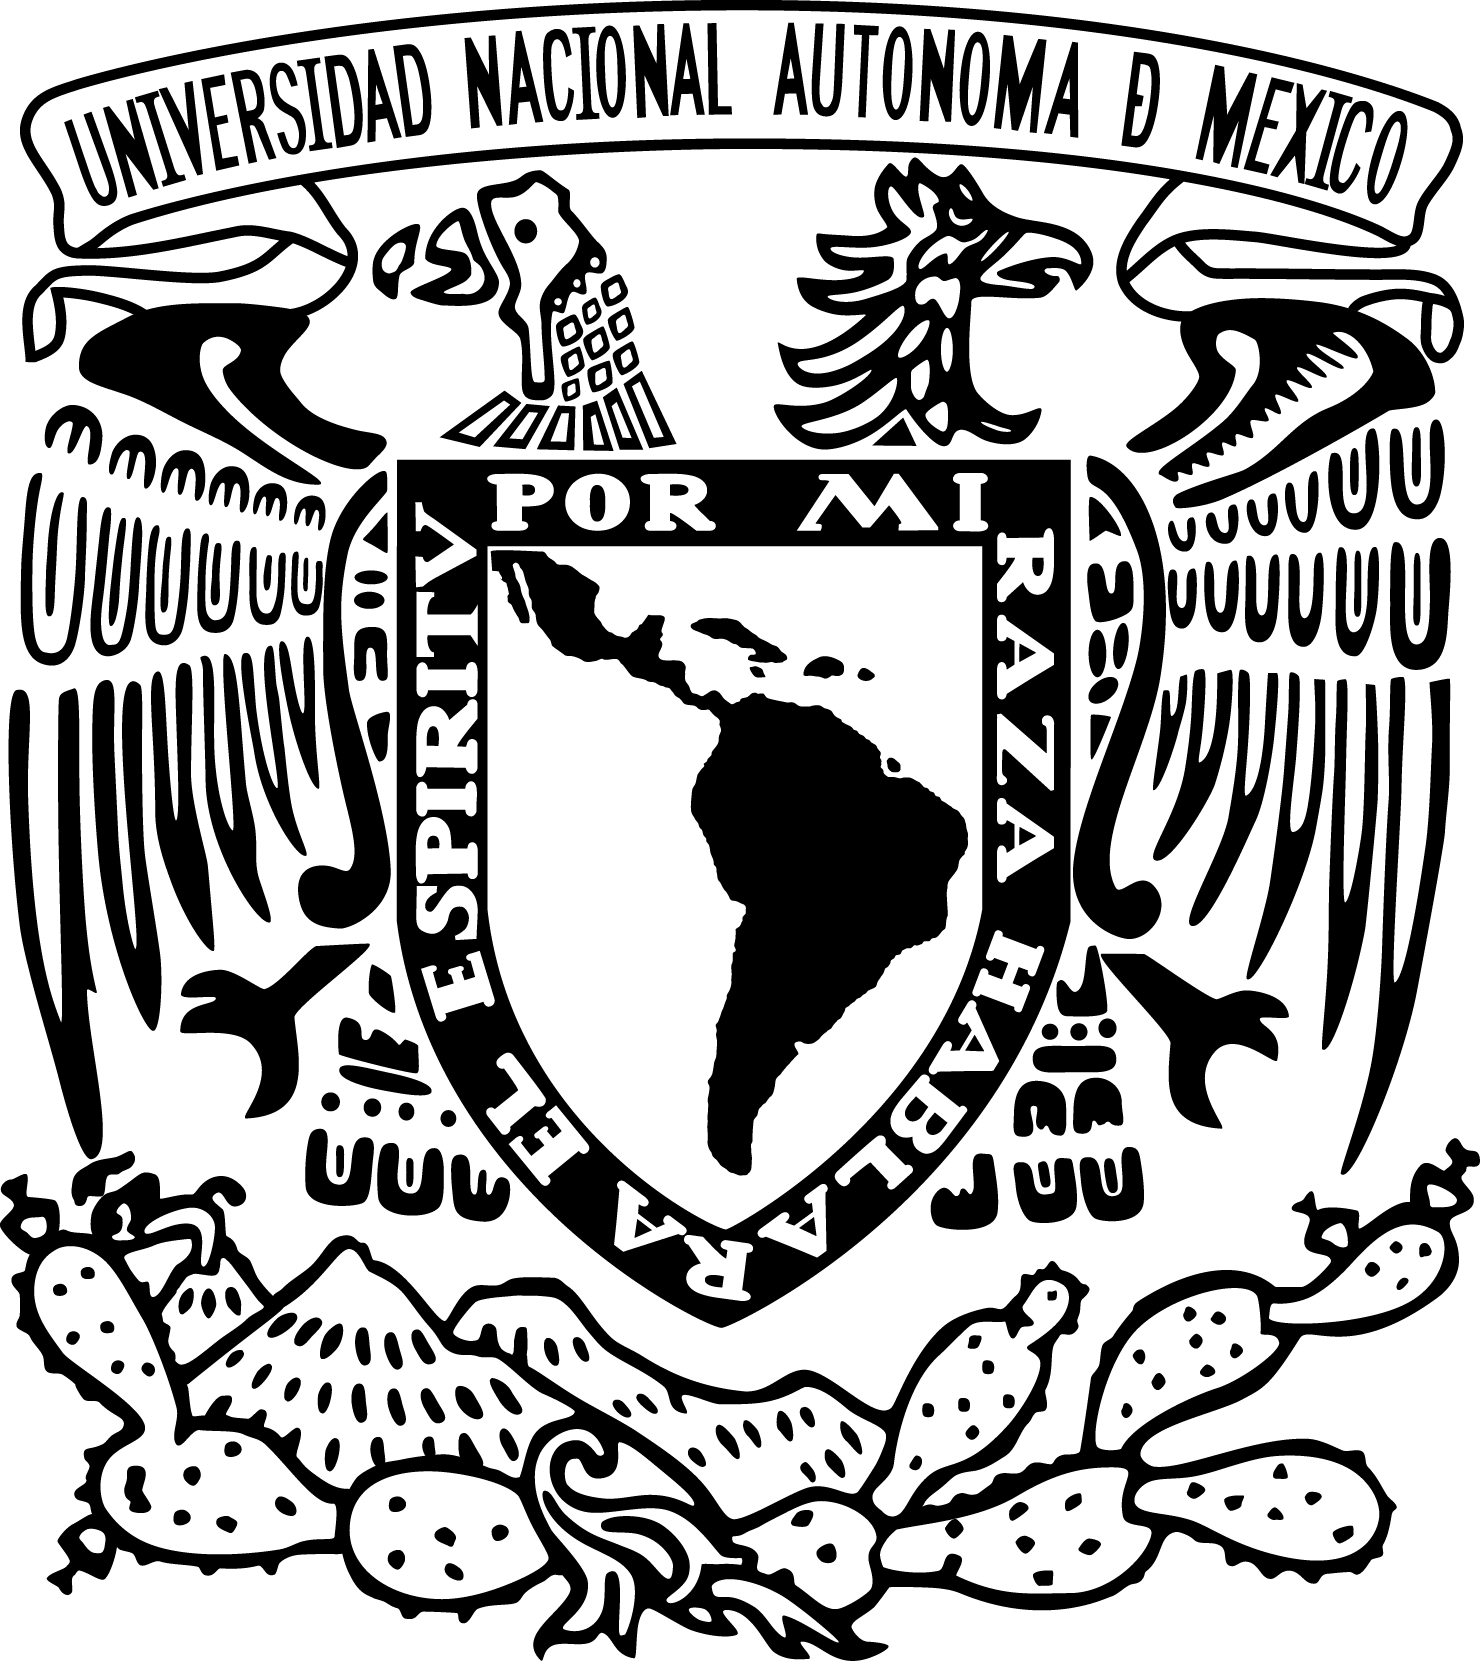
\includegraphics[height=1.5cm]{unam-escudo.png}}

\logo{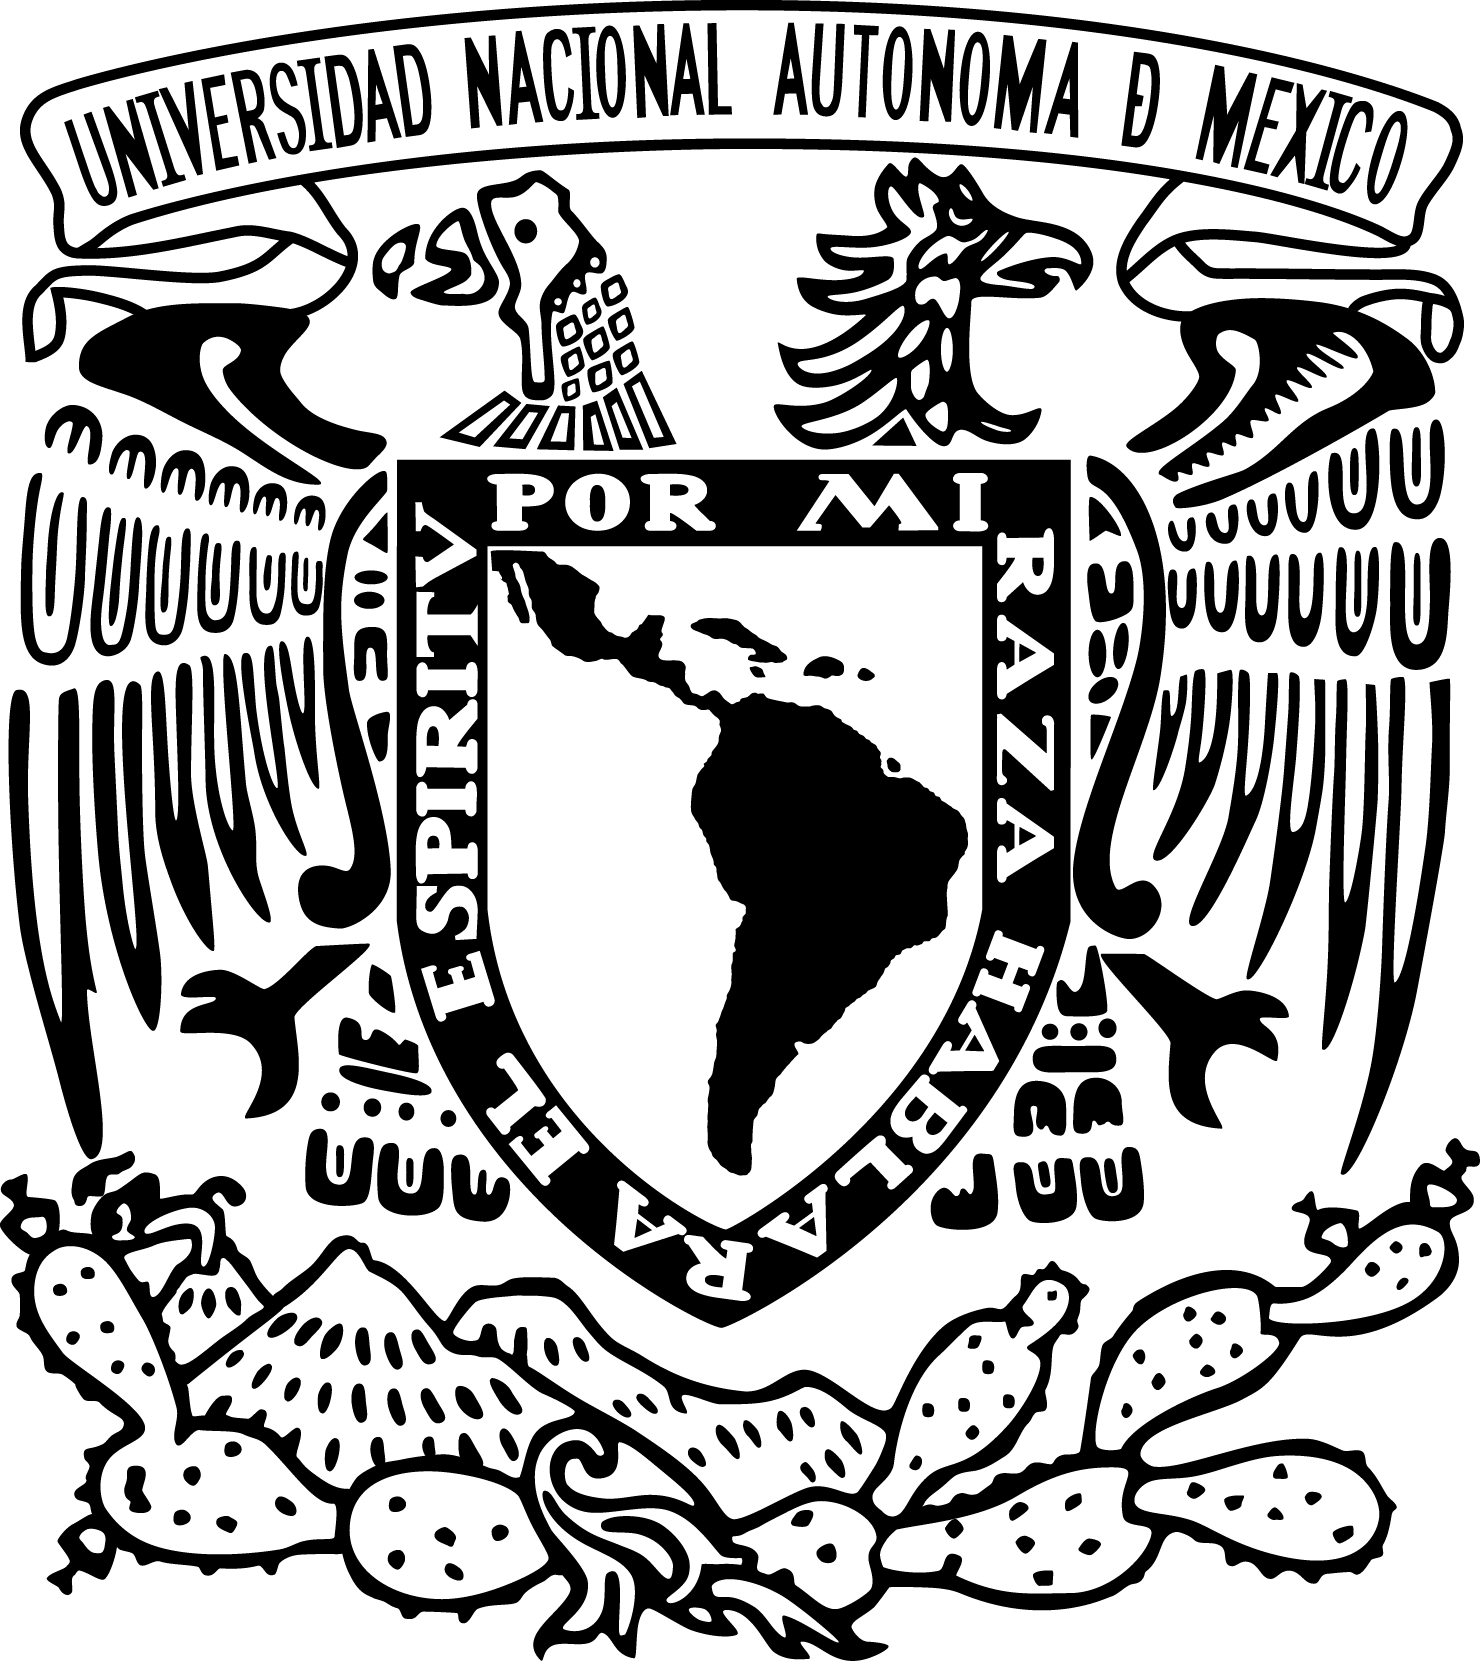
\includegraphics[height=0.8cm]{unam-escudo.png}\hspace{12pt}\vspace{-13pt}}
%\hspace{11cm}\vspace{-25pt}}  
      
\begin{document}

\maketitle

\begin{frame}{Contenido}
  \setbeamertemplate{section in toc}[sections numbered]
  \tableofcontents[hideallsubsections]
\end{frame}

\section{Introducción}

\begin{frame}{Sistemas complejos}

	\begin{itemize}
	\item<1->[$\blacksquare$]Los \textbf{sistemas complejos} están conformados por una gran cantidad de componentes interactuando mutuamente entre sí. 
	\item<2->[$\blacksquare$]George Zipf \textcolor{BrickRed}{\hyperlink{bibliografia}{[1]}} trató a los idiomas como sistemas complejos.
	\only<2>{$$ f(k)\sim \frac{1}{k} $$}
	
	\item<3->[$\blacksquare$]Actualmente es evidente el empleo de palabras inglesas.
	
	\item<4>[$\blacksquare$]La mezcla de palabras entre idiomas, originó este trabajo.  
	
	\end{itemize}

\end{frame}

\begin{frame}[fragile]{Objetivos}
	\begin{enumerate}
		\item \textbf{\large{Determinar y cuantificar la influencia de una lengua en otra.}}
	\end{enumerate}
\end{frame}


\begin{frame}[fragile]{Base de datos}
	
	\begin{itemize}
		\only<1-2>{\item[$\blacksquare$]Las publicaciones en los idiomas inglés, francés, alemán, italiano y español, en 269 años (1740-2009) obtenidas de Google Books \textcolor{BrickRed}{\hyperlink{bibliografia}{[2]}}.}
		\vspace{1cm}
		\only<2>{\item[$\blacksquare$]Por cada año y por cada idioma se tomaron las 5 mil palabras más usadas.}
		%\item<3>[$\blacksquare$]Cada palabra esta asociada a una frecuencia y un rango.	
	\end{itemize}
	
	\only<3>{	
		\begin{columns}
			\column[t]{4cm}    %new code
			\begin{itemize}
				\vspace{1cm}
				\item[$\blacksquare$]Cada palabra esta asociada a una frecuencia $f$ y un rango $k$.	
			\end{itemize}
			
			\column[t]{.5\textwidth}    %new code
			\begin{exampleblock}{Estructura de una lista}
				\begin{tabular}{ccc}
					\multicolumn{3}{c}{\textbf{Año $t$}}          \\
					Rango $k$     & Palabra    & Frecuencia $f$    \\
					1             & pal 1      & $f_{1}$            \\
					2             & pal 2      & $f_{2}$             \\
					3             & pal 3      & $f_{3}$              \\
					$\vdots$      & $\vdots$   & $\vdots$         \\
					$\vdots$      & $\vdots$   & $\vdots$         \\
					$5000$        & pal $5000$ & $f_{5000}$          
				\end{tabular}
			\end{exampleblock}
			
		\end{columns}
	}
\end{frame}

\begin{frame}[fragile]{Definiciones y forma de búsqueda}
	\begin{itemize}
		\item<1->[$\blacksquare$]Las \textbf{palabras migrantes} son palabras que están presentes en al menos dos idiomas y con igual escritura, carácter por carácter.
		\item<2->[$\blacksquare$]El \textbf{idioma origen} es aquel donde proviene la palabra migrante.
		\item<3>[$\blacksquare$]El \textbf{idioma receptor} es aquel donde la palabra está presente.		
	\end{itemize}	
\end{frame}

\begin{frame}[fragile]{Limpieza de datos}
	No se consideraron 
	\begin{itemize}
		\item<2->[$\blacksquare$] Palabras funcionales.
		\\ 
		\centering\textcolor{Sepia}{\textit{él, hacía, para.}}
		\\
		\item<3->[$\blacksquare$] Palabras combinadas con carácteres numéricos.
		\\
		\centering\textcolor{Sepia}{\textit{pag177}}
		\\
		\item<4->[$\blacksquare$] Palabras que aparecen sólo una vez en el idioma receptor.
	\end{itemize}
	
\end{frame}

\section{Préstamos nuevos}


\begin{frame}[fragile]{Definición}
	
	Los \textbf{préstamos nuevos} son palabras que aparecen por primera vez en las cinco mil más usadas del idioma receptor.
	
	%Un \textbf{campo semántico} es un conjunto de palabras asociadas que comparten parte de su significado. 
\end{frame}

\begin{frame}{Préstamos nuevos del inglés }
		\begin{columns}
			\visible<1->{
			\column[t]{.5\textwidth}
			\begin{figure}[h!]
				\centering
				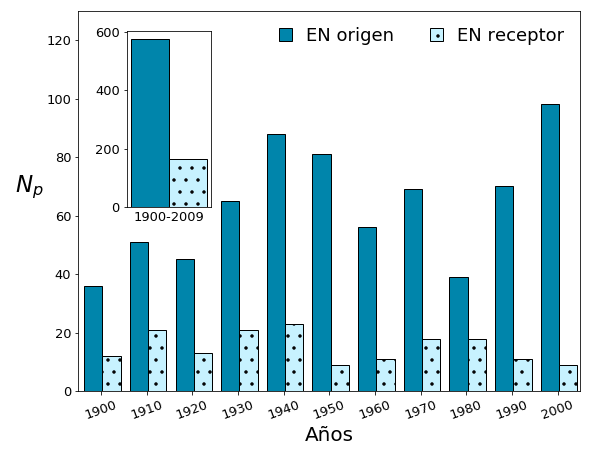
\includegraphics[width=\columnwidth]{BOR_EN.png}
			\end{figure}
			}
		
			\column[t]{.5\textwidth} 
			\\	
			\visible<2->{
			\textcolor{Sepia}{Segunda Guerra Mundial.}
			\begin{itemize}
				\item churchill, catastrophe (1940)  
			\end{itemize} 
			
			\textcolor{Sepia}{Tecnología}
			\begin{itemize}
				\item internet, online, mail, software (1990 y 2000)
			\end{itemize}
			
			\textcolor{Sepia}{Globalización}
			\begin{itemize}
				\item standars, market, value, customer (1980, 1900, 2000)
			\end{itemize}
			}
		\end{columns}
	
\end{frame}


\begin{frame}{Préstamos nuevos de los demás idiomas}
\vspace{5mm}
\makebox[\textwidth]{%
	\begin{tabular}{c c}
		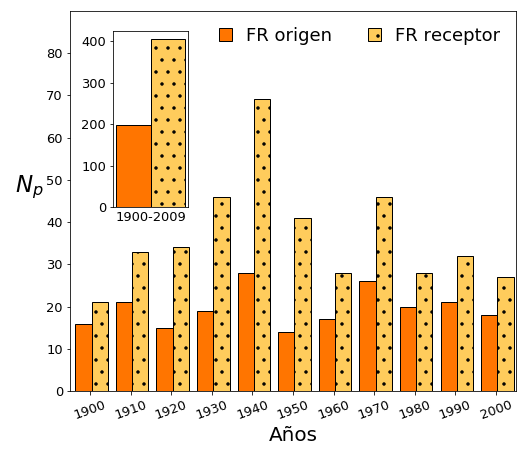
\includegraphics[width=4.0cm,height=3.5cm]{BOR_FR.png} &
		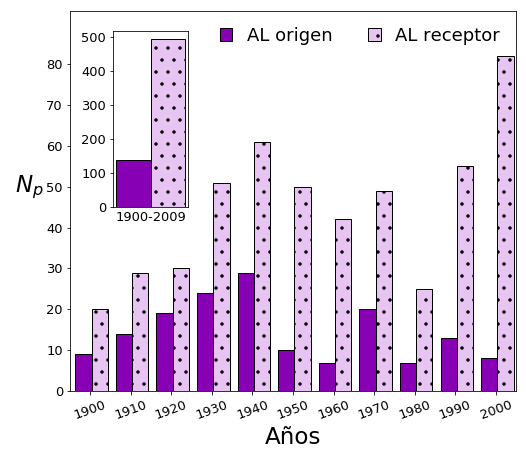
\includegraphics[width=4.0cm,height=3.5cm]{BOR_GE.png} \\
		\vspace{5mm}
		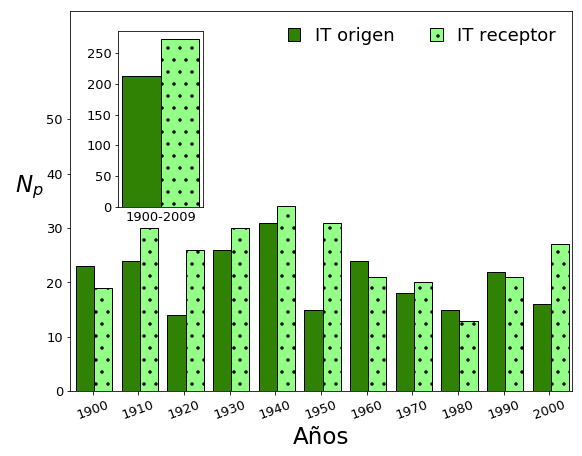
\includegraphics[width=4.0cm,height=3.5cm]{BOR_IT.png} &
		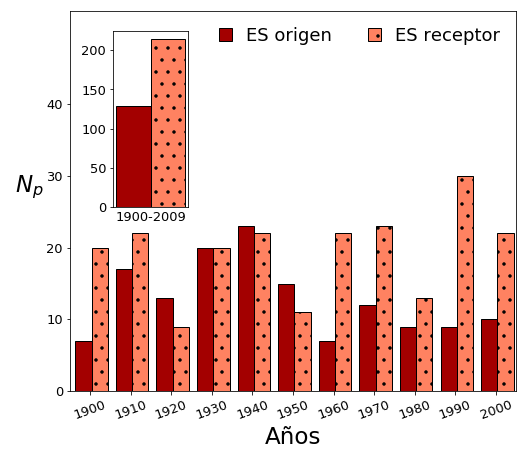
\includegraphics[width=4.0cm,height=3.5cm]{BOR_SP.png} \\

	\end{tabular}%
}
\end{frame}

\begin{frame}[fragile]{Resultados de los préstamos nuevos}
	\begin{itemize}
		\item<1->[$\blacksquare$]\large{Las palabras migran de un idioma a otro tras ocurrir un evento histórico o cultural.}\\
		
		\item<2>[$\blacksquare$]\large{Las palabras migrantes se pueden agrupar en campos semánticos.} 
		
		\begin{itemize}
			\item Inglés: guerra, política, tecnología y globalización.
			\item Francés: guerra, política y apellidos académicos.
			\item Alemán: guerra y apellidos académicos.
			\item Italiano: guerra e ideologías políticas.
			\item Español: medicina y nombres de países Latinoamericanos. 
		
		\end{itemize}
	\end{itemize}
\end{frame}


\section{Préstamos acumulados}


\begin{frame}[fragile]{Características}
	
	\visible<1->{$\blacksquare$ Un \textbf{préstamo acumulado} es una palabra con origen $A$ que ya había aparecido en un receptor $B$, y para un determinado año lo vuelve a hacer.}
	
	\visible<2->{$\blacksquare$ Los préstamos nuevos se vuelven acumulados si aparecen posterior a su año de migración.}
	
	%\visible<3>{
	%	\centering
	%	\begin{tabular}{lcccccc}
	%		\multicolumn{7}{c}{R E C E P T O R}                                                                                                                                             \\
	%		\multirow{6}{*}{\begin{tabular}[c]{@{}l@{}}O\\ R\\ \,I\\ G\\ E\\ N\end{tabular}} &             & \textbf{inglés} & \textbf{francés} & \textbf{alemán} & \textbf{italiano} & \textbf{español} \\
	%		& \textbf{inglés}   & -           & 6.48$\%$  & 3.28$\%$      & 1.55$\%$   & 1.47$\%$    \\
	%		& \textbf{francés}  & 5.94$\%$    & -         & 1.88$\%$      & 2.37$\%$   & 1.32$\%$    \\
	%		& \textbf{alemán}   & 1.27$\%$    & 1.28$\%$  & -             & 0.69$\%$   & 0.30$\%$    \\
	%		& \textbf{italiano} & 1.55$\%$    & 2.01$\%$  & 0.95$\%$      & -          & 4.38$\%$    \\
	%		& \textbf{español} & 2.36$\%$     & 1.68$\%$  & 0.50$\%$      & 6.23$\%$    & -          
	%	\end{tabular}
	%}
	
\end{frame}

\begin{frame}[fragile]{El uso entre idiomas}
	
	%Para un año $t$, si $k$ es el rango de las cinco mil palabras, y $j$ el rango de los préstamos acumulados.
	
	Para un año $t$, si $j$ representa el rango de los préstamos acumulados y $k$ el rango de las cinco mil palabras del idioma receptor, entonces:
	
	\visible<2->{
	$$ \underset{ \text{\tiny A} \to  \text{\tiny B} }{U}(t) = \frac{\sum_{j} f(j)}{\sum_{k=1}^{5000} f(k)}. $$
	}
	
\end{frame}

\begin{frame}{El uso del inglés en los demás idiomas}
	\visible<1->{
		\begin{center}
			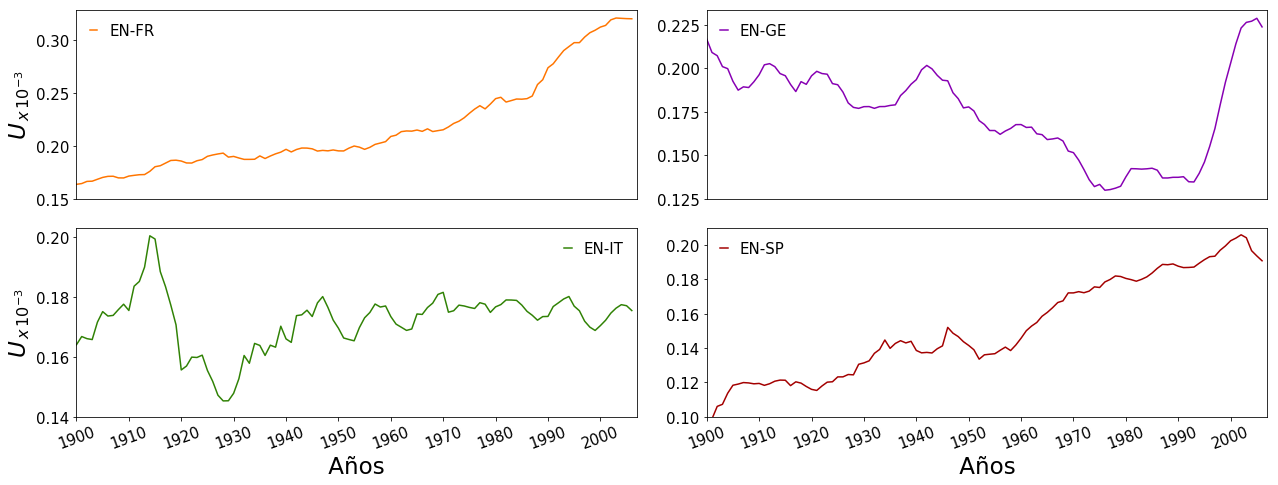
\includegraphics[width=\textwidth]{UO1_EN.png}
		\end{center}
	}
	\visible<2->{Mayor influencia en el alemán (1990-2003).
	}
	
	\vspace{3mm}
	\visible<3->{
		\begin{columns}
			\column[b]{.4\textwidth}
			\textcolor{Sepia}{Tecnología}
			\begin{itemize}
				\item internet, software, digital.
			\end{itemize}
			
			\column[b]{.4\textwidth} 
			\textcolor{Sepia}{Globalización}
			\begin{itemize}
				\item investment, marketing, company.
			\end{itemize}
		\end{columns}
	}
	%\only<5>{\textcolor{Sepia}{Industria vitivinícola}
	%	\begin{itemize}
	%		\item raisins, vin, vignoble, recolte.
	%	\end{itemize}
	%}
\end{frame}

\begin{frame}{El uso del francés en los demás idiomas}
	\visible<1->{
		\begin{center}
			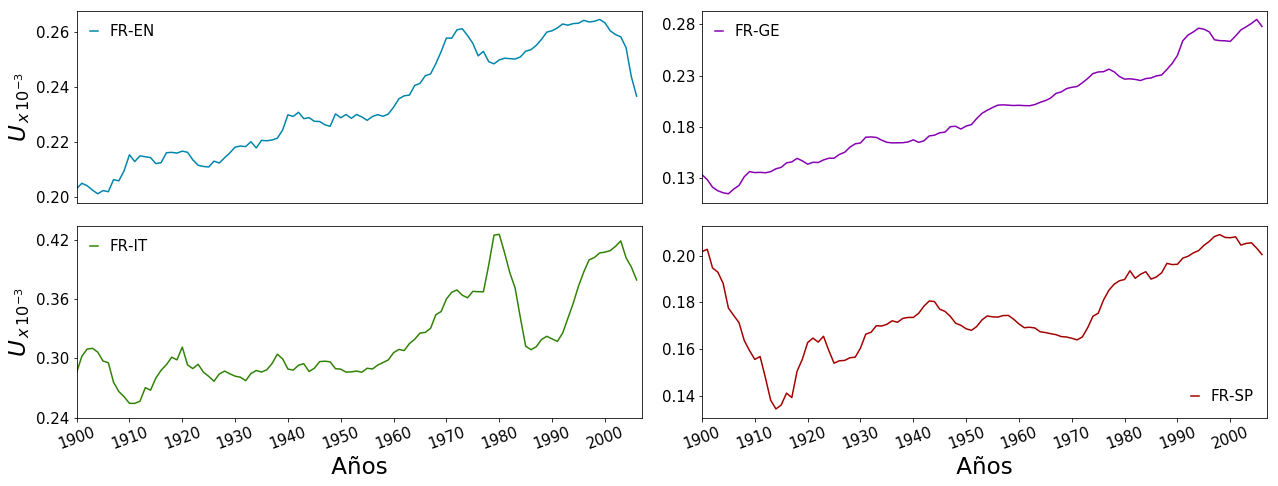
\includegraphics[width=\textwidth]{UO1_FR.png}
		\end{center}
		}
	\visible<2->{Mayor influencia en el italiano (1950-1970).
	}
	
	\vspace{3mm}
	\visible<3->{
	\begin{columns}
		\column[b]{.4\textwidth}
		\textcolor{Sepia}{Revolución Francesa}
		\begin{itemize}
			\item bastille, bourgeois, napoleon, imperiale 
		\end{itemize}
	
		\column[b]{.4\textwidth} 
		\textcolor{Sepia}{Religión}
		\begin{itemize}
			\item saint, eglise, dime
		\end{itemize}
	\end{columns}
	}
	%\only<5>{\textcolor{Sepia}{Industria vitivinícola}
	%	\begin{itemize}
	%		\item raisins, vin, vignoble, recolte.
	%	\end{itemize}
	%}
\end{frame}
%{
%\begin{frame}
%	\only<1->{
%		\begin{center}
%			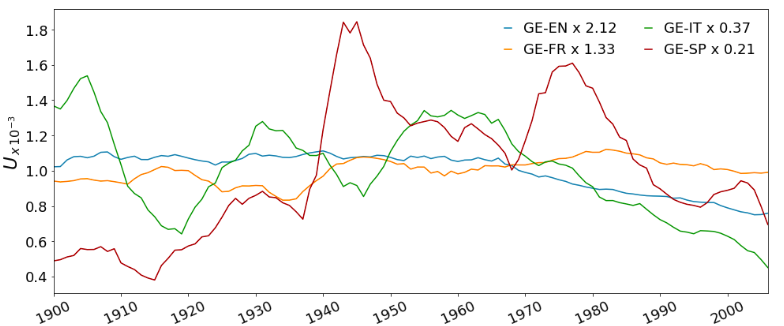
\includegraphics[height=4.5cm]{GE_UOR.png}
%		\end{center}
%		
%		Mayor Uso: Español 0.0021 fpa (1935-1945),  inglés -0.00015 (1960-2009).
%	}
%	\\
%	\only<2>{\textcolor{Sepia}{Segunda Guerra Mundial.}
%		\begin{itemize}
%			\item berlin, hitler, reich, testen.
%		\end{itemize}
%	}
%	\only<3>{\textcolor{Sepia}{Apellidos académicos}
%		\begin{itemize}
%			\item marz, freud, heideggger, nietzsche, hegel, engels. 
%		\end{itemize}
%	}
	
%\end{frame}

%\begin{frame}
%	\only<1->{
%		\begin{center}
%			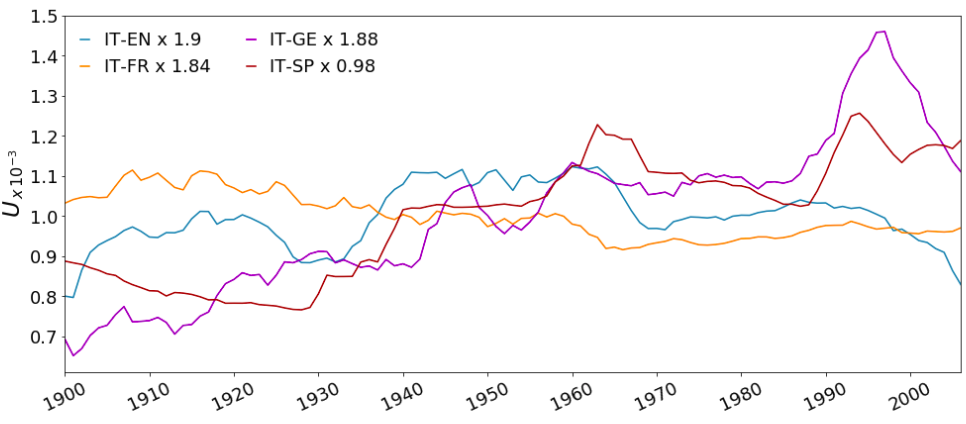
\includegraphics[height=4.5cm]{IT_UOR.png}
%		\end{center}
%		
%		Mayor Uso: Inglés 0.0035 fpa (1930-1940), español 0.0011 fpa (1930-1960).
%	}
%	\\
%	\only<2>{\textcolor{Sepia}{Segunda Guerra Mundial.}
%		\begin{itemize}
%			\item mussolini, fascismo, battlagia.
%		\end{itemize}
%	}
%	\only<3>{\textcolor{Sepia}{Religión}
%		\begin{itemize}
%			\item santo, suora, cattedrale. 
%		\end{itemize}
%	}
	
%\end{frame}

\begin{frame}{Resultados sobre los préstamos acumulados}
	\begin{itemize}
		
		\item<1->[$\blacksquare$]\large{La influencia se relaciona con un  cambio en el uso entre idiomas.} %un periodo de tiempo donde el uso de un idioma en otro cambia.
		
		\item<2>[$\blacksquare$]\large{Tras un suceso histórico o cultural habrá un aumento en la influencia, y estarán involucradas palabras de ciertos campos semánticos.} 
		
		%Si el uso aumenta en los años alrededor de un suceso, las palabras de un campo semántico aumentarán su frecuencia.

	\end{itemize}
\end{frame}


\section{Robustez} 

\begin{frame}[fragile]{Errores en las clasificaciones}
	
	\only<1->{
	Problemas:}
	\begin{itemize}
		\item <1->[$\blacksquare$] Hay errores en las palabras migrantes.
		\begin{itemize}
			\item Igual escritura y diferente significado: \textcolor{Sepia}{\textit{mayor}}
		\end{itemize}
	
		\item <2->[$\blacksquare$]No sabemos detectarlos de forma practica.
			
		\item <3->[$\blacksquare$]Ni cómo afecta una limpieza al uso entre idiomas.
	\end{itemize}
	
	\visible<4->{
	Propuesta:}
	\begin{itemize}
		\item<4-> [$\blacksquare$] Eliminar una porcentaje de los préstamos acumulados y calcular el uso reducido.
		
		\item<5-> [$\blacksquare$] Necesitamos una medida de similitud, entre el uso original y el uso reducido.
		\visible<6>{
		$$
		\left\langle D \right\rangle  = \frac{1}{N}\sum_{t=1}^{N} \left| u_{t} - r_{t} \right|.
		$$
		}
	\end{itemize}
\end{frame}

\begin{frame}{Eliminación por rangos}
	
	\visible<2->{
	\begin{minipage}{2cm}
		$\blacksquare$ Rangos\\
		\vspace{1mm}$\,\,\,\,\,\,$ bajos.
	\end{minipage}%
	\begin{minipage}{11cm}
		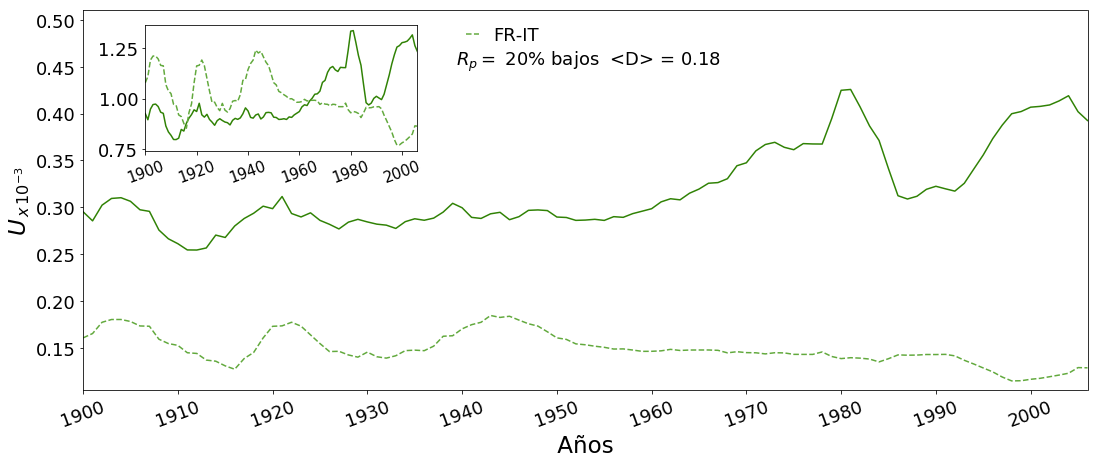
\includegraphics[height=3.5cm]{OM_FI1.png}
	\end{minipage}
	}
	\hfill
	\visible<3->{
	\begin{minipage}{2cm}
		$\blacksquare$ Rangos \\ 
		\vspace{1mm} $\,\,\,\,\,$ altos.
	\end{minipage}%
	\begin{minipage}{11cm}
		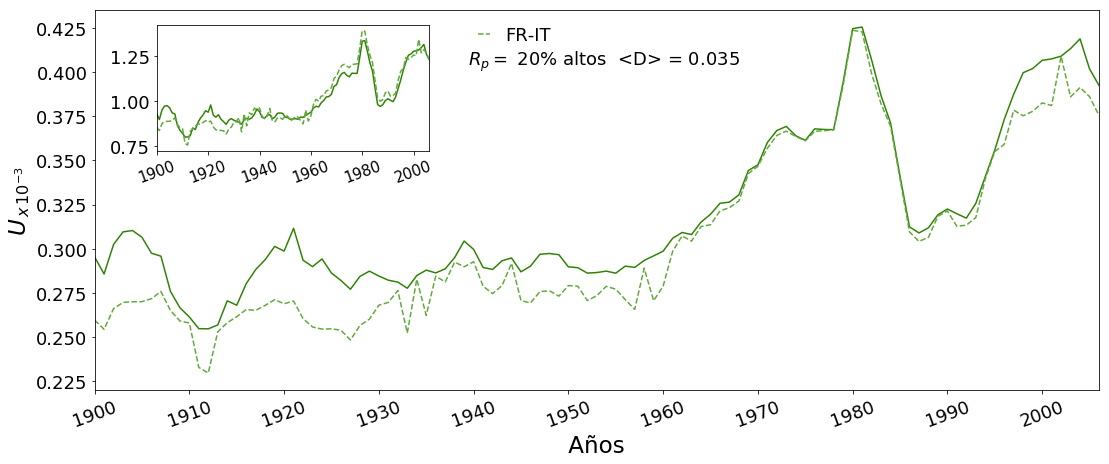
\includegraphics[height=3.5cm]{OM_FI2.png}
	\end{minipage}
	}

\end{frame}

\begin{frame}{¿Qué tanto podemos eliminar?}
	
	\begin{columns}
		\column[t]{.5\textwidth}
		\visible<2->{
			$\blacksquare$ Rangos bajos 
			\begin{figure}[t]
				\centering
				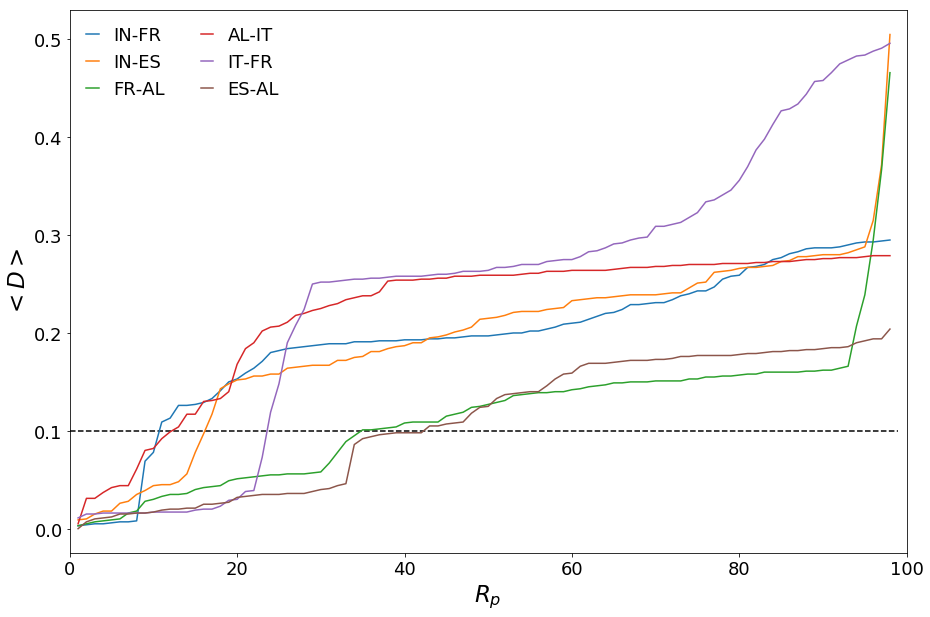
\includegraphics[width=5.25cm, height=4.25cm]{OM_bajos.png}
			\end{figure}
		}
		
		\column[t]{.5\textwidth}
		\visible<3->{
			$\blacksquare$ Rangos altos 
			\begin{figure}[t]
				\centering
				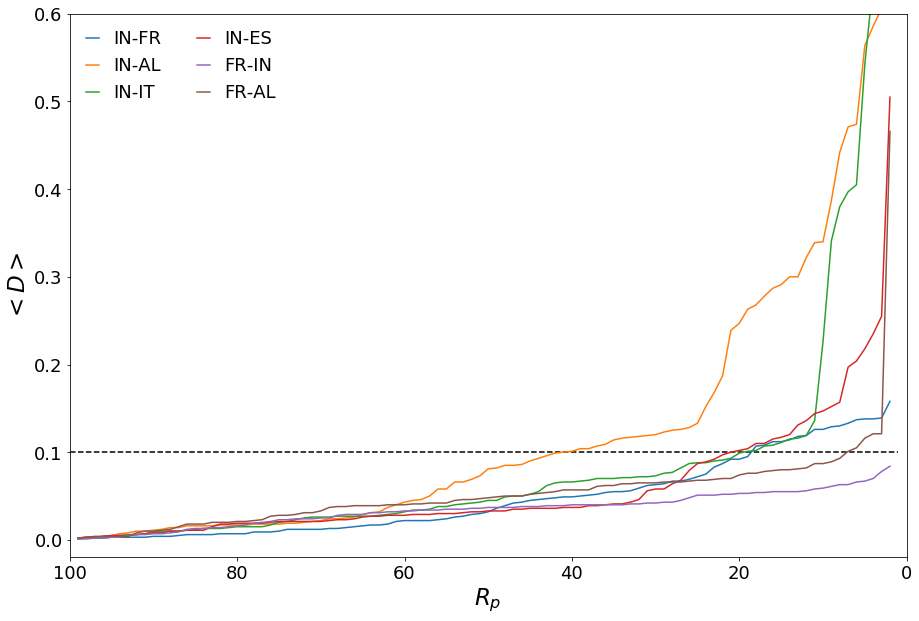
\includegraphics[width=5.25cm, height=4.25cm]{OM_altos.png}
			\end{figure}
		}
	\end{columns}
	
	\visible<4->{
		\begin{itemize}
			\item<4-> [$\blacksquare$]\large{El peso del uso entre idiomas, lo llevan las palabras con los rangos bajos.} 
			
			\item<5-> [$\blacksquare$]\large{El método es bueno si en las palabras más frecuentes hay pocos errores de clasificación.}
		\end{itemize}
	}
	
\end{frame}






\section{Diversidad de rango}

\begin{frame}{Motivación}
	\begin{itemize}
	\item<1->[$\blacksquare$] Comprender qué tan diferentes son las palabras que ocupan un mismo rango $k$ a lo largo del tiempo.
	%\item<2->[$\blacksquare$] ¿Que tanto modifican su rango los préstamos acumulados?
	\vspace{5mm}
	\item<2->[$\blacksquare$]La diversidad de rango $d(k)$ cuantifica tal situación. 
	\end{itemize}
\end{frame}


%\begin{frame}{Ajuste a una curva logarítmica}
%	
%	\begin{figure}[t]
%		\centering
%		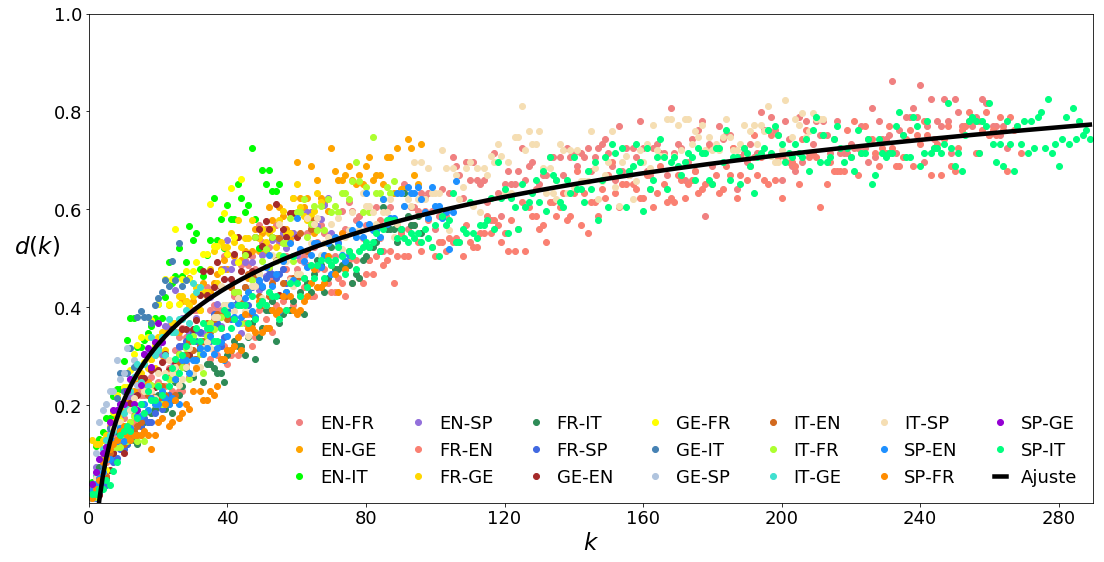
\includegraphics[height=4.5cm]{DR_gen.png}
%	\end{figure}
%	\vspace{0.5mm}
%	$$d(k) = 0.16\ln(k) - 0.17. $$
%
%	\begin{itemize}
%	\item<2->[$\blacksquare$] Fácil de calcular.
%	\item<3>[$\blacksquare$]  No es fiable en rangos bajos.  %          $R^{2} = \left [0.79, 0.95  \right ]$.
%	\end{itemize}

%\end{frame}

\begin{frame}{Ajuste a una curva sigmoide}
		\begin{columns}
		\visible<1->{
		\column[]{.6\textwidth}
		\centering
		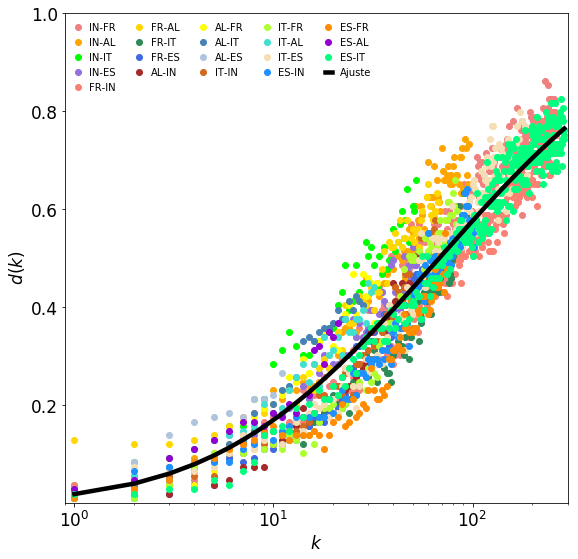
\includegraphics[height=5.3cm, width =6.4cm]{DR_sig.png}
		}
		\visible<2->{
		\column[]{.5\textwidth} 
		$$d(k) = \frac{1}{\sigma\sqrt{2\pi}}\int_{-\infty }^{\log_{10^{k}}} e^{-\frac{\left ( y-\mu \right )^{2}}{2\sigma^{2}}}dy.$$ 	
		\\
		$$ \mu = 1.83\,\,\,\,\,\sigma = 0.87$$
		} 
	\end{columns}
	
	\visible<3->{
	\begin{itemize}
		\item<3->[$\blacksquare$] El ajuste es fiable, en promedio $R^{2}=0.95$.
		\item<4>[$\blacksquare$] Concuerda con los resultados  hechos en idiomas~\textcolor{BrickRed}{\hyperlink{bibliografia}{[3]}}, y en deportes y juegos~\textcolor{BrickRed}{\hyperlink{bibliografia}{[4]}}.
	\end{itemize}
	}
\end{frame}

\begin{frame}{Resultados de la diversidad}
	\begin{itemize}
		\item<1->[$\blacksquare$]\large{ La diversidad de palabras que pueden ocupar un mismo rango, aumenta conforme el rango también lo hace.}
		\\
		\item<2> [$\blacksquare$] \large{Este comportamiento  es valido sin importar el tamaño del corpus.}
	\end{itemize}

\end{frame}

\section{Conclusiones}

\begin{frame}{Conclusiones}
\only<1-3>{
	\begin{itemize}
	\item<1->[$\blacksquare$] \large{Las migraciones de palabras y el aumento de la influencia entre idiomas, son provocadas por eventos históricos o culturales.}
	%\item<2-4>[$\blacksquare$] El suceso tambien  hará que las palabras de su campo semantico aumenten su frecuencia.
	%\item<2->[$\blacksquare$] Los idiomas influyen más que otros en ciertas areas.
	\item<2->[$\blacksquare$]\large{ Los errores en las clasificaciones pueden ser  despreciables si estos están en los rangos más altos.}
	
	\item<3>[$\blacksquare$]\large{A lo largo del tiempo, la diversidad de palabras que pueden ocupar un mismo rango, aumenta conforme el rango también lo hace.}
	\end{itemize}
	}
		
	\only<4>{
	\begin{itemize}
	\item<4> \large{\textbf{Inglés:} guerra, política, tecnología y globalización.}
	\item<4> \large{\textbf{Francés:} guerra, política, religión, industria vitivínicola  y apellidos académicos.}
	\item<4> \large{\textbf{Alemán:} guerra y apellidos académicos.}
	\item<4> \large{\textbf{Italiano:} guerra e ideologías políticas.}
	\item<4> \large{\textbf{Español:} medicina y nombres de países Latinoamericanos.} 
	\end{itemize}
	}


\end{frame}

\begin{frame}[plain, noframenumbering]{Bibliografía}
	\label{bibliografia}
	\begin{thebibliography}{10}
		\setbeamertemplate{bibliography item}[text]
		
		\bibitem{1} Zipf G.K. \textit{Selective Studies and the Principle of Relative Frequency in Language.} Harvard University Press., Cambridge, MA, USA., 1932.
		
		\\
		
		\bibitem{2} Google Books. \textbf{N Gram Viewer}, 2019. [Online, accesado 12-06-2019]. Disponible en: \href{https://books.google.com/ngrams}{\textcolor{RoyalBlue}{https://books.google.com/ngrams}}.
		
		\\
		%\bibitem{3} COCHO G., FLORES J., GERSHENSON C., PINEDA C., AND SÁNCHEZ S.
		\bibitem{3} Cocho G., Flores J., Gershenson C., Pineda C., and Sánchez S., \textbf{Diversity of Languages: Generic Behavior in Computational Linguistics}. \textit{PLoS ONE 10(4): e0121898}, 2015
		Disponible en: \href{https://doi.org/10.1371/journal.pone.0121898}{\textcolor{RoyalBlue}{ https://doi.org/10.1371/journal.pone.0121898.}}
		
		\\
		
		%\bibitem{4} MORALES J.A, SÁNCHEZ S., FLORES J., GERSHENSON C., PINEDA C., COCHO G., ZIZUMBO J., RODRÍGUEZ R.F., AND IÑIGUEZ G.
		\bibitem{4} Morales J.A., Sánchez S., Flores J., Pineda C., Gershenson C., Cocho G., Zizumbo J., Rodríguez R.F., and Iñiguez G. 
		\textbf{Generic temporal features of performance rankings in sports and games}. \textit{EPJ Data Sience 33(5)}, 2016. Disponible en: \href{https://doi.org/10.1140/epjds/s13688-016-0096-y}{\textcolor{RoyalBlue}{https://doi.org/10.1140/epjds/s13688-016-0096-y.}} 

	\end{thebibliography}
\end{frame}


%\begin{frame}[noframenumbering]{Bibliografía}
%	\printbibliography
%\end{frame}

\end{document}